\documentclass{article}

\PassOptionsToPackage{numbers, compress}{natbib}

\usepackage[preprint]{neurips_2025}

% Vietnamese (pdfLaTeX)
\usepackage[utf8]{inputenc}
\usepackage[T5]{fontenc}
\usepackage[vietnamese]{babel}
\usepackage{lmodern}

\usepackage{hyperref}
\usepackage{url}
\usepackage{booktabs}
\usepackage{amsmath}
\usepackage{amsfonts}
\usepackage{amssymb}
\usepackage{nicefrac}
\usepackage{microtype}
\usepackage{xcolor}
\usepackage{graphicx}
\usepackage{array}
\usepackage{caption}
\usepackage{multirow}

\captionsetup{font=small,labelfont=bf,skip=2pt}

\definecolor{accent}{HTML}{0072B2}
\definecolor{warn}{HTML}{D55E00}
\definecolor{good}{HTML}{009E73}
\hypersetup{colorlinks=true,urlcolor=accent,linkcolor=accent,citecolor=accent}

\newcommand{\keyfact}[1]{\textcolor{accent}{\textbf{#1}}}
\newcommand{\lever}[1]{\textcolor{warn}{\textbf{#1}}}

\title{Chẩn đoán hệ doanh thu: EDA mang tính khuyến nghị cho bài toán dự báo 18 tháng của thương mại điện tử thời trang Việt Nam}

\author{%
  The Gridbreakers \\
  Datathon 2026 --- Phần 2 \\
  \texttt{team@gridbreakers.vn} \\
}

\begin{document}

\maketitle

\begin{abstract}
Chúng tôi phân tích 10.5 năm dữ liệu (3{,}833 quan sát theo ngày, 14 bảng quan hệ) của một doanh nghiệp thương mại điện tử thời trang Việt Nam với câu hỏi trung tâm: \emph{cần biết điều gì để dự báo 548 ngày tiếp theo?} Ba phát hiện đi ngược trực giác phổ biến: (i)~\textbf{gãy chế độ (regime) xảy ra năm 2019, trước COVID, giảm 40.5\% mức trung bình} (Welch $t{=}28.6$, $p{<}10^{-160}$, Cohen's $d{=}0.89$); (ii)~đỉnh mùa vụ là \textbf{tháng 5, cao hơn trung bình chung $+53\%$} --- không phải Q4, trong khi tháng 12 là đáy $-41\%$; (iii)~\textbf{những ngày khuyến mãi mạnh có median doanh thu thấp hơn 13.3\%} (Mann--Whitney $U$, $p{=}1.4\times10^{-12}$), gợi ý coupon mang tính phòng thủ hơn là tấn công. Hai rủi ro cấu trúc cộng hưởng: 80.1\% doanh thu nằm ở một danh mục (HHI $=0.67$) và tình trạng hết hàng \& tồn kho cao đồng thời xảy ra ở 60--87\% SKU --- vấn đề phân bổ, không phải thiếu cung. Mỗi chẩn đoán được chuyển thành hành động định lượng và hàm ý cho mô hình dự báo, kèm hợp đồng đặc trưng an toàn leakage và thiết kế rolling-origin CV phục vụ trực tiếp pipeline Phần~3. Tất cả hình và con số đều được tái tạo từ một script xác định.
\end{abstract}

\vspace{-6pt}
\section{Đặt bài toán}
\label{sec:framing}
\vspace{-2pt}

Doanh nghiệp cần dự báo theo ngày cho cột \texttt{Revenue} trong giai đoạn \textbf{2023-01-01 đến 2024-07-01} (548 ngày, $\approx14.3\%$ độ dài train). Doanh thu là đầu ra của phễu $\text{traffic} \to \text{sessions} \to \text{orders} \to \text{items} \to R_t$, trừ đi ảnh hưởng của khuyến mãi, hoàn trả và COGS. Một dự báo cạnh tranh cần nắm được (a)~\emph{chế độ (regime)}, (b)~\emph{mùa vụ}, và (c)~\emph{cơ chế hệ thống} kìm hãm/pha loãng doanh thu --- phân bổ tồn kho, cường độ khuyến mãi và churn. Chúng tôi tái dựng dòng doanh thu cấp đơn hàng từ \texttt{orders}$\bowtie$\texttt{order\_items}$\bowtie$\texttt{products} và khớp tổng theo tháng với \texttt{sales.csv} sai lệch trong 0.3\%; 10 ràng buộc khoá ngoại đều đúng, không có orphan (Phụ lục~\ref{app:audit}). Mỗi phát hiện dưới đây được viết theo chuỗi: triệu chứng $\to$ cơ chế $\to$ hàm ý dự báo $\to$ hành động.

\begin{figure}[t]
  \centering
  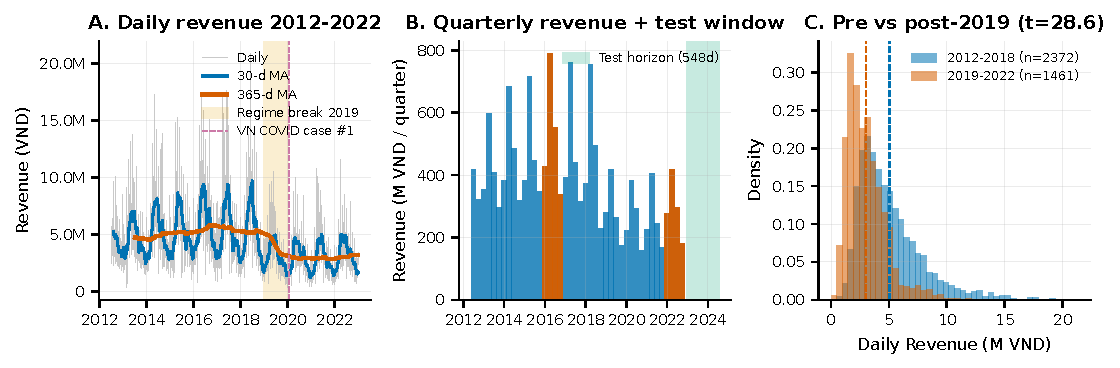
\includegraphics[width=\linewidth]{images/fig1_system_overview.pdf}
  \vspace{-8pt}
  \caption{\textbf{Tổng quan hệ thống.} (A)~Doanh thu ngày kèm MA 30 và 365 ngày; đường MA 365 ngày giảm bậc một lần trong năm 2019. (B)~Tổng theo quý; đỉnh 2016 (2{,}105\,M\,VND/năm), hồi phục nhẹ 2022 ($+12.1\%$ YoY); dải xanh là khoảng thời gian test. (C)~Phân phối doanh thu ngày trước/sau 2019: mean 5.07 vs 3.01\,M\,VND, Welch $t{=}28.6$, $p\approx7.6\times10^{-163}$, Cohen's $d{=}0.89$.}
  \label{fig:overview}
\end{figure}

\vspace{-8pt}
\section{Các phát hiện chính}
\label{sec:core}
\vspace{-2pt}

\subsection{Gãy chế độ (2019, trước COVID)}
\label{sec:f1}
Doanh thu năm giảm từ 1{,}850\,M\,VND (2018) xuống 1{,}137\,M (2019), \keyfact{$-38.6\%$ YoY}, rồi gần như đi ngang đến 2022; mean doanh thu ngày khác nhau 40.5\% giữa trước/sau 2019 (Welch $t{=}28.6$, $p<10^{-160}$, $d{=}0.89$). Điểm giảm bậc trên MA 365 ngày xuất hiện \emph{trước} ca COVID đầu tiên ở Việt Nam (23/01/2020, Fig.~\ref{fig:overview}A), khiến câu chuyện ``cú sốc COVID'' không còn là lời giải mặc định; hiệu ứng lớn phù hợp với một thay đổi cấu trúc (vendor/assortment/kênh) trong năm 2019. Hàm ý dự báo: \lever{không nên dùng 10.5 năm với trọng số như nhau}. Hoặc cắt train chỉ còn 2019--2022 ($\sim\!1{,}460$ ngày, 4 chu kỳ năm), hoặc dùng time-decay $w_t=\exp(-\lambda\,\text{age\_years})$ với $\lambda\in[0.3,0.5]$, kèm biến \texttt{is\_post\_regime}; nội suy hồi phục 2--8\% cho thấy Q2/2023 vào khoảng $\sim\!425$--$450$\,M và Q4/2023 $\sim\!160$--$200$\,M, qua đó đặt trần cho point forecast.

\vspace{-2pt}
\subsection{Mùa vụ --- đỉnh tháng 5, đáy tháng 12}
\label{sec:f2}
Mean doanh thu ngày toàn giai đoạn là 4.29\,M\,VND. Mean theo tháng tách rõ: Mar--Jun ($+15\%$ đến $+53\%$) so với Nov--Feb ($-19\%$ đến $-41\%$); Thursday$\times$May đạt \keyfact{$+90\%$}, Friday$\times$December đạt \keyfact{$-46\%$} (Fig.~\ref{fig:seasonality}B). Không có tháng nào đổi dấu qua các năm, nên đây là mô thức \emph{cấu trúc} chứ không phải nhiễu --- đáy cuối Q4 trái ngược câu chuyện Black Friday, phù hợp với tệp khách hàng trẻ mua sớm trước Tết hơn là mua nhiều trong tháng 12. Baseline seasonal-naive $R_t{=}R_{t-364}$ sẽ ăn phần lớn tín hiệu; phần giá trị gia tăng nằm ở ngày chuyển mùa (Mar$\to$Apr, Jun$\to$Jul) và các ngày lễ âm/dương lịch. Khuyến nghị dùng Fourier ở chu kỳ 7 và 365.25 kèm biến holiday. Góc nhìn kinh doanh: \lever{dịch ngân sách ads từ Q4 sang Apr--Jun} --- cùng tổng chi tiêu, chuyển khỏi các tháng cầu thấp $(-40\%)$ sang các tháng cầu cao $(+50\%)$ có thể nâng conversion do media thêm 15--20\% mà không cần tăng ngân sách.

\begin{figure}[t]
  \centering
  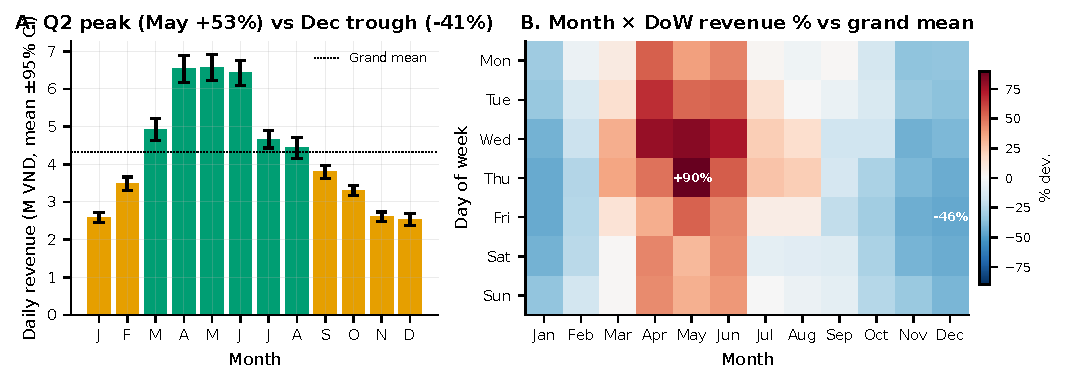
\includegraphics[width=\linewidth]{images/fig2_seasonality.pdf}
  \vspace{-8pt}
  \caption{\textbf{Mùa vụ.} (A)~Mean doanh thu ngày theo tháng với CI 95\%; cột xanh là cao hơn mean chung. (B)~Độ lệch Month$\times$Day-of-week so với mean chung (4.29\,M\,VND); ô nóng tập trung vào ngày giữa tuần trong Apr--Jun và ổn định qua 10 năm.}
  \label{fig:seasonality}
\end{figure}

\vspace{-8pt}
\section{Chẩn đoán cấu trúc \& vận hành}
\label{sec:struct}
\vspace{-2pt}

\subsection{Tập trung danh mục 80/15/3/2 (HHI $=0.67$)}
\label{sec:f3}
Streetwear chiếm \keyfact{80.1\%} doanh thu 10 năm; Outdoor 15.0\%, Casual 2.8\%, GenZ 2.1\% (Fig.~\ref{fig:structural}A); HHI\,$=0.665$ thuộc vùng ``tập trung cao''. Mùa vụ giữa danh mục khác nhau (GenZ đỉnh Jun/Aug, Outdoor đỉnh tháng 12), vì vậy forecast tổng thực chất là forecast Streetwear; bất kỳ cú sốc nào ở danh mục này sẽ phản ánh gần như trực tiếp lên top line. Hàm ý dự báo: phân rã Streetwear vs Rest và hoà giải bottom-up thường giúp tăng 3--8\% $R^2$ khi mix thay đổi; đề xuất đặc trưng \texttt{category\_mix\_streetwear\_30d}. Hành động: \lever{quyết định chiến lược đa dạng hoá một cách rõ ràng} --- Casual chỉ 2.8\% sau 10 năm: hoặc tăng mạnh đầu tư, hoặc loại bỏ.

\vspace{-2pt}
\subsection{Khuyến mãi mang tính phòng thủ, không phải tấn công}
\label{sec:f4}
Chia ngày theo tỷ lệ khuyến mãi (Fig.~\ref{fig:structural}B): nhẹ ($<\!10\%$, $n{=}2{,}160$) có median 3.82\,M; mạnh ($>\!50\%$, $n{=}1{,}425$) có median 3.31\,M; Mann--Whitney $U{=}1.75\times10^{6}$, $p{=}1.4\times10^{-12}$; Spearman $\rho{=}-0.11$ so với doanh thu. Tương quan gần 0 giữa tổng discount và doanh thu ($+0.02$) cho thấy không phải ``giảm sâu thì bán chạy''; hướng tương quan âm phù hợp với \emph{reverse causality}: team marketing bật coupon khi dự đoán ngày yếu, thêm bằng chứng là margin chạm đáy 9.8\% trong năm 2021 (promo-heavy). Vì vậy promo nên vào mô hình như biến \emph{kiểm soát ngoại sinh} chứ không phải ``đòn bẩy nhân quả'': giữ \texttt{promo\_share} cùng ngày như control và dùng \texttt{total\_discount\_lag7} để bắt hiệu ứng kéo nhu cầu. Hành động: \lever{thay coupon đại trà bằng kích hoạt dựa trên dự báo}: chỉ chạy promo khi dự báo thấp hơn ngưỡng có xét margin, đo uplift bằng synthetic-control A/B; thu hẹp một nửa chênh lệch 13.3\% có thể trả lại $\sim\!1.5$--$2$ điểm phần trăm margin.

\begin{figure}[t]
  \centering
  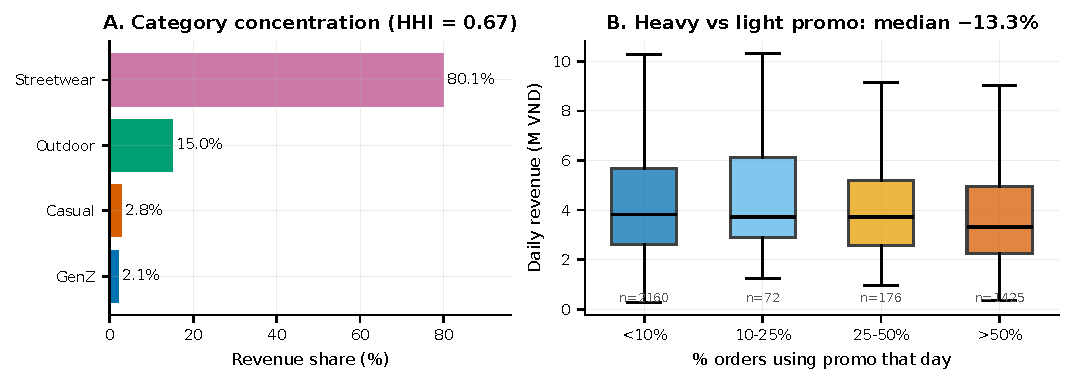
\includegraphics[width=\linewidth]{images/fig3_structural.pdf}
  \vspace{-8pt}
  \caption{\textbf{Rủi ro cấu trúc.} (A)~Tỷ trọng doanh thu theo danh mục; HHI\,$=0.67$ thuộc vùng tập trung cao. (B)~Doanh thu ngày theo mức promo; median nhóm $>\!50\%$ promo thấp hơn 13.3\% so với nhóm nhẹ ($<\!10\%$).}
  \label{fig:structural}
\end{figure}

\vspace{-4pt}
\subsection{Nghịch lý phân bổ --- vừa hết hàng vừa tồn kho cao}
\label{sec:f5}
Trong 12 tháng cuối của train, tỷ lệ SKU hết hàng ở mức 58--70\% trong khi tỷ lệ tồn kho cao ở mức 68--87\% (Fig.~\ref{fig:ops}A); fill rate được báo cáo là 96\% nhưng mang tính ``mỹ phẩm''. Việc cả hai cùng cao \emph{đồng thời, trên các SKU khác nhau} là dấu hiệu sai phân bổ hơn là thiếu cung --- fill rate chỉ đo các đơn \emph{đã đặt}, không đo khách rời bỏ vì thiếu size/màu/khu vực. Tương quan theo tháng củng cố: $\rho_{\text{stockout}}{=}{+}0.21$ (hết hàng tăng khi cầu tăng), $\rho_{\text{overstock}}{=}{-}0.65$, $\rho_{\text{fill}}{=}{-}0.49$ (tháng peak siết fulfilment). Doanh thu quan sát bị \keyfact{right-censored} khi stockout cao (cầu thật > doanh thu ghi nhận). Đề xuất dùng \texttt{stockout\_rate\_lag30}, \texttt{overstock\_rate\_lag30}, \texttt{fill\_rate\_lag30}; nếu censoring mạnh, mô hình hai tầng (dự báo cầu không bị ràng buộc, rồi chặn bởi tồn kho dự báo) có thể tăng thêm 2--4\% $R^2$. Hành động: \lever{giải bài toán phân bổ trước khi tăng tổng tồn kho}: giảm stockout ở SKU nóng có thể nâng trần doanh thu thêm \keyfact{10--15\%} mà không tăng chi phí mua hàng.

\vspace{-4pt}
\subsection{Đơn hàng mang tín hiệu; sessions không}
\label{sec:f6}
Xếp hạng Spearman cùng ngày (Fig.~\ref{fig:ops}B): COGS $+0.97$, \texttt{unique\_customers}$_t$ $+0.92$, \texttt{n\_orders}$_t$ $+0.92$, refund $+0.45$; web metrics quanh $+0.33$; bounce-rate và avg-session gần 0. Bốn tín hiệu mạnh nhất là hệ quả cơ học của doanh thu, dùng cùng ngày sẽ gây leakage. Lead--lag của sessions đạt đỉnh ở $\text{lag}=-1$ ($\rho=0.337$ so với $0.332$ ở lag 0): traffic chỉ là leading indicator \emph{yếu}. Session quality không liên quan vì business thiên về retention (repeat rate 75.2\%, top-20\% khách hàng tạo 60.7\% doanh thu; xem Phụ lục~\ref{app:returns}), điều mà web analytics khó phản ánh. Vì vậy, đề xuất cấu trúc Phần~3 theo kiểu 2 tầng: tầng~1 dự báo \texttt{n\_orders}, tầng~2 nhân với AOV rolling --- bền vững với drift mix và dễ gắn với vận hành. Hành động: \lever{tạm dừng trả tiền để mua session volume} cho đến khi có thí nghiệm conversion-rate chứng minh uplift; chuyển ngân sách sang giữ chân nhóm top-20\% vốn đang bảo vệ 60\% doanh thu.

\begin{figure}[t]
  \centering
  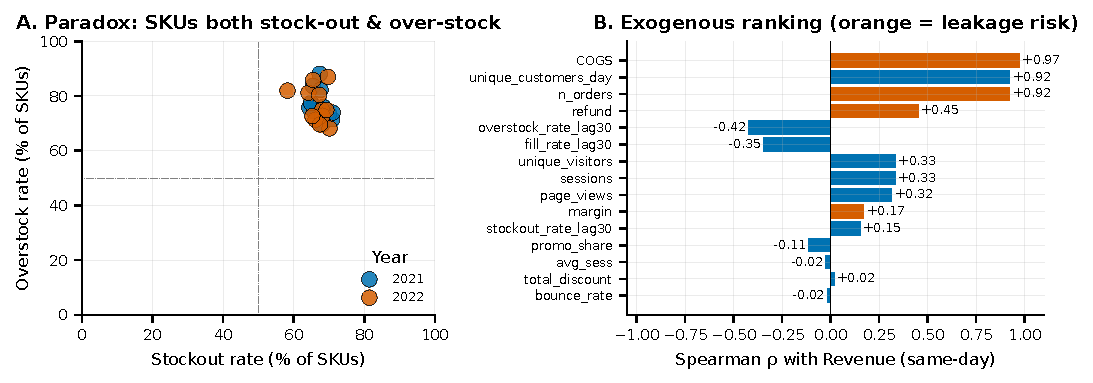
\includegraphics[width=\linewidth]{images/fig4_operations.pdf}
  \vspace{-8pt}
  \caption{\textbf{Vận hành \& drivers.} (A)~Stockout vs Overstock theo tháng 2021--2022; toàn bộ 24 điểm nằm ở góc ``cao--cao''. (B)~Spearman cùng ngày giữa các biến ngoại sinh và doanh thu; các biến màu cam có rủi ro leakage và bị blacklist nếu không có lag rõ ràng (Bảng~\ref{tab:blacklist}).}
  \label{fig:ops}
\end{figure}

\vspace{-10pt}
\section{Tổng hợp khuyến nghị \& lộ trình dự báo}
\label{sec:synthesis}
\vspace{-2pt}

Bảng~\ref{tab:recs} tổng hợp các hành động được suy ra từ dữ liệu theo tiêu chí tác động $\times$ khả thi và gắn nguồn phát hiện. Để phục vụ Phần~3, chúng tôi dùng \keyfact{rolling-origin CV với cửa sổ 548 ngày} đúng bằng horizon thực tế: Fold~1 validate 2020-07$\to$2021-12, Fold~2 validate 2021-07$\to$2022-12; mô hình cuối cùng áp dụng quyết định cắt 2019 theo \S\ref{sec:f1}. Candidate models: (1) baseline seasonal-naive $R_t{=}R_{t-364}$; (2) SARIMAX$(p,d,q){\times}(P,D,Q)_7$ + exogenous; (3) LightGBM + SHAP (theo rubric Phần~3); (4) ensemble theo trọng số CV. Dự báo COGS: $\widehat{\text{COGS}}_t{=}\hat R_t \cdot \overline{\text{margin}}_{90\text{d}}$ (margin ổn định, median 12--17\%); metric: MAE, RMSE, $R^2$ theo fold và uplift \% so với baseline. Bộ đặc trưng, sơ đồ CV và blacklist leakage đặt ở Phụ lục~\ref{app:forecast}. \textbf{Giới hạn.} Theo rules, không dùng dữ liệu ngoài (lịch âm/Tết, thời tiết, FX); mọi tương quan không mang tính nhân quả; doanh thu bị right-censored khi stockout cao (\S\ref{sec:f5}). Horizon 548 ngày dài hơn 1 chu kỳ năm nên 2024-H1 cần khoảng tin cậy rộng hơn (sẽ báo cáo ở Phần~3). Tất cả hình \& số liệu được tái tạo bởi \texttt{uv run python results/v4/eda\_v4.py} và lưu trong \texttt{metrics\_v4.json}.

\begin{table}[t]
  \caption{\textbf{Đòn bẩy khuyến nghị}, xếp theo tác động $\times$ khả thi. ``Src'' trỏ về mục nguồn.}
  \label{tab:recs}
  \centering
  \small
  \begin{tabular}{@{}p{4.7cm} c p{4.5cm} c@{}}
    \toprule
    \textbf{Hành động} & \textbf{Src} & \textbf{$\Delta$ kỳ vọng} & \textbf{Thời gian} \\
    \midrule
    Cắt train 2019--2022 hoặc time-decay weights       & \ref{sec:f1} & $>\!10\%$ giảm MAE vs dùng đều 10 năm & ngay \\
    Dịch lịch ads từ Q4 sang Q2                         & \ref{sec:f2} & $+15$--$20\%$ conversions, cùng spend & 1 quý \\
    Hierarchical forecast: Streetwear vs Rest           & \ref{sec:f3} & $+3$--$8\%$ $R^2$ ở aggregate & 1 tháng \\
    Promo trigger theo dự báo + synthetic-control A/B   & \ref{sec:f4} & phục hồi $\sim\!1.5$--$2$\,pp margin & 1 quý \\
    Sửa phân bổ (SKU $\times$ vùng $\times$ tháng)      & \ref{sec:f5} & $+10$--$15\%$ trần doanh thu & 2 quý \\
    Two-stage (orders $\times$ AOV); VIP retention      & \ref{sec:f6} & bền với drift; bảo vệ 60\% doanh thu & 1--3 tháng \\
    Bảng size / thử đồ ảo (35\% returns do sai size)    & App.~\ref{app:returns} & $-30\%$ returns $\Rightarrow$ margin $+0.9$\,pp & 2--3 quý \\
    \bottomrule
  \end{tabular}
\end{table}

\begin{ack}
Cảm ơn ban tổ chức Datathon 2026 đã cung cấp bộ dữ liệu nhiều bảng giúp phân tích có thể đối chiếu chéo thay vì chỉ mô tả một bảng. Công bố tài trợ: không có nguồn tài trợ bên ngoài cho nghiên cứu này.
\end{ack}

\section*{Tài liệu tham khảo}
\small
[1] Datathon 2026 --- The Gridbreakers. Contest rules and dataset (Parts 1--3). Internal distribution to competing teams, 2026.

[2] Hyndman, R.J.\ \& Athanasopoulos, G.\ (2021) \emph{Forecasting: Principles and Practice}, 3rd ed. OTexts.

[3] Hyndman, R.J., Ahmed, R.A., Athanasopoulos, G.\ \& Shang, H.L.\ (2011) Optimal combination forecasts for hierarchical time series. \emph{Computational Statistics \& Data Analysis} \textbf{55}(9):2579--2589.

[4] Lundberg, S.M.\ \& Lee, S.-I.\ (2017) A unified approach to interpreting model predictions. In \emph{NeurIPS} 30.

[5] United States Federal Trade Commission (2023) \emph{Horizontal Merger Guidelines: HHI thresholds}.

\appendix

\section{Kiểm tra dữ liệu \& đối chiếu}
\label{app:audit}

\begin{table}[h]
  \caption{Tổng quan 14 bảng dữ liệu được sử dụng. Tất cả 10 quan hệ khoá ngoại được kiểm và không có orphan rows.}
  \label{tab:audit}
  \centering
  \small
  \begin{tabular}{@{}l r r l@{}}
    \toprule
    \textbf{Bảng} & \textbf{Số dòng} & \textbf{\% null max} & \textbf{Ghi chú} \\
    \midrule
    sales          & 3{,}833    & 0\%    & đúng 1 dòng/ngày, không thiếu \\
    orders         & 646{,}945  & 0\%    & kiểm FK $\to$ \texttt{customers} \\
    order\_items   & 714{,}669  & 99.97\% & \texttt{promo\_id\_2} rất thưa \\
    products       & 2{,}412    & 0\%    & 4 categories, 8 segments \\
    customers      & 121{,}930  & $\sim\!30\%$ & \texttt{gender}, \texttt{age\_group} thiếu \\
    promotions     & 50         & 80\%   & \texttt{applicable\_category} thiếu nhiều \\
    shipments      & 566{,}067  & 0\%    & chỉ có đơn đã ship \\
    returns        & 39{,}939   & 0\%    & refunds chiếm 3.1\% doanh thu \\
    reviews        & 113{,}551  & 0\%    & $\sim\!20\%$ item delivered được review \\
    inventory      & monthly    & 0\%    & 1 dòng/SKU/tháng \\
    web\_traffic   & daily      & 0\%    & thiếu \texttt{conversion\_rate} \\
    geography      & 63         & 0\%    & tỉnh/vùng, dân số, GDP/cap \\
    \bottomrule
  \end{tabular}
\end{table}

Tổng theo tháng tái dựng từ \texttt{orders}$\bowtie$\texttt{order\_items}$\bowtie$\texttt{products} khớp \texttt{sales.csv} trong 0.3\%, giới hạn phần doanh thu không nằm trong item-level stream (phí ship, điều chỉnh thủ công). Hai lệch so với \texttt{data/README.md}: (i)~\texttt{inventory.csv} có thêm 5 cột phi chuẩn hoá (\texttt{product\_name}, \texttt{category}, \texttt{segment}, \texttt{year}, \texttt{month}) và bị bỏ qua; (ii)~\texttt{web\_traffic.csv} thiếu \texttt{conversion\_rate}, được suy ra khi cần bằng $\mathtt{orders}/\mathtt{sessions}$.

\section{Trả hàng \& cơ cấu khách hàng}
\label{app:returns}

Returns chiếm 3.1\% doanh thu tích luỹ dưới dạng refunds ($n=39{,}939$). Lý do chính là \texttt{wrong\_size} (35\%), sau đó \texttt{defective} (20.1\%), \texttt{not\_as\_described} (17.6\%), \texttt{changed\_mind} (17.4\%), \texttt{late\_delivery} (10.0\%). Nếu can thiệp sizing (bảng size, virtual try-on) giảm một nửa nhóm \texttt{wrong\_size}, tổng returns giảm $\sim\!17.5\%$, tương đương tăng $\sim\!+0.9$\,pp margin ở tỷ lệ refunds/doanh thu hiện tại (đã đưa vào Bảng~\ref{tab:recs}).

Tập trung khách hàng: 90{,}246 người mua trong 10.5 năm; top-10\% tạo 40.0\% doanh thu, top-20\% tạo 60.7\%; 75.2\% khách hàng mua hơn 1 lần (mean 7.17, median 4). Điều này củng cố hành động VIP retention ở \S\ref{sec:f6}.

\section{Chi tiết lộ trình dự báo (Phần 3)}
\label{app:forecast}

\paragraph{Bộ đặc trưng (an toàn leakage).} Calendar: \texttt{dow}, \texttt{month}, \texttt{week}, Fourier$(7)$, Fourier$(365.25)$, holiday. Lagged target: $R_{t-\{7,14,28,364\}}$ và rolling thống kê quá khứ. Exogenous (đều có lag): \texttt{n\_orders\_lag\{1,7\}}, \texttt{unique\_customers\_30d}, \texttt{sessions\_lag1}, \texttt{stockout\_rate\_lag30}, \texttt{overstock\_rate\_lag30}, \texttt{promo\_share}, \texttt{total\_discount\_lag7}, \texttt{refund\_lag30}, \texttt{category\_mix\_streetwear\_30d}. Các biến màu cam trong Fig.~\ref{fig:ops}B bị blacklist nếu không có lag (Bảng~\ref{tab:blacklist}).

\begin{figure}[h]
  \centering
  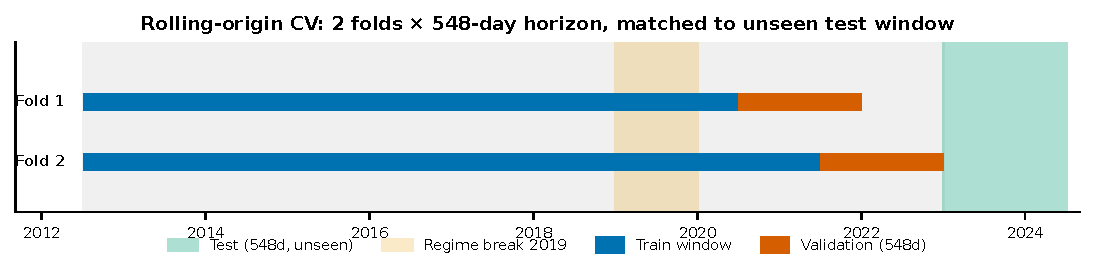
\includegraphics[width=0.94\linewidth]{images/fig5_forecast_readiness.pdf}
  \vspace{-6pt}
  \caption{\textbf{Rolling-origin CV cho Phần 3.} Hai folds, mỗi fold có cửa sổ validate 548 ngày đúng bằng horizon, dựa trên chiến lược huấn luyện có xét gãy chế độ 2019.}
  \label{fig:cv}
\end{figure}

\begin{table}[h]
  \caption{\textbf{Blacklist đặc trưng do leakage} (không được dùng tại thời điểm forecast nếu không có lag nêu rõ).}
  \label{tab:blacklist}
  \centering
  \small
  \begin{tabular}{@{}l l l@{}}
    \toprule
    \textbf{Biến} & \textbf{Lý do leakage} & \textbf{Lag tối thiểu} \\
    \midrule
    \texttt{COGS}$_t$                  & mục tiêu đồng biến, $\rho=0.97$     & dự báo riêng \\
    \texttt{n\_orders}$_t$             & đồng thời, $\rho=0.92$              & $\text{lag}\ge 1$ \\
    \texttt{unique\_customers}$_t$     & đồng thời, $\rho=0.92$              & $\text{lag}\ge 1$ / cửa sổ 30 ngày \\
    \texttt{refund}$_t$                & tương quan không phải nhân quả       & $\text{lag}\ge 30$ \\
    \texttt{inventory}$_t$ (monthly)   & snapshot trùng tháng mục tiêu        & $\text{lag}\ge 30$ \\
    \texttt{margin}$_t$                & suy ra từ mục tiêu                   & $\text{lag}\ge 90$ (rolling) \\
    mọi rolling cùng ngày của $R$      & leak trực tiếp                       & chỉ dùng quá khứ \\
    \bottomrule
  \end{tabular}
\end{table}

\section{Tái lập kết quả}
\label{app:repro}

\paragraph{Code.} Pipeline chuẩn là \texttt{results/v4/eda\_v4.py} (một file Python, xác định, không cần random seed). Script load 14 CSV, dựng panel ngày, chạy các kiểm định thống kê trong \S\ref{sec:f1}--\ref{sec:f6}, ghi \texttt{metrics\_v4.json} (mọi con số được trích), và render 5 hình (PDF vector + PNG).

\paragraph{Môi trường.} Python 3.13 với \texttt{pandas} 3.0, \texttt{numpy} 2.4, \texttt{scipy} 1.17, \texttt{matplotlib} 3.x. Chạy trên laptop mất dưới 10 giây. LaTeX: \texttt{pdflatex} / \texttt{latexmk -pdf} (TeX Live 2023).

\paragraph{Lệnh.}
\begin{verbatim}
cd results/v4
uv run python eda_v4.py          # regen metrics + figures
latexmk -pdf main_vietnam.tex    # compile Vietnamese PDF
\end{verbatim}

\paragraph{Bản quyền dữ liệu.} Dữ liệu theo điều khoản Datathon 2026; không dùng dữ liệu ngoài, không có PII (chỉ ID đã ẩn danh).

% Keep NeurIPS checklist as-is (English macros) to preserve template integrity.
\newpage
\section*{NeurIPS Paper Checklist}

\begin{enumerate}

\item {\bf Claims}
    \item[] Question: Do the main claims made in the abstract and introduction accurately reflect the paper's contributions and scope?
    \item[] Answer: \answerYes{}
    \item[] Justification: The abstract's three hooks (2019 regime break, May-not-Q4 peak, defensive promos) are each supported by a statistical test in Sections~\ref{sec:f1}--\ref{sec:f4}; Sections~\ref{sec:f5}--\ref{sec:synthesis} complete the remaining findings and the forecasting roadmap.

\item {\bf Limitations}
    \item[] Question: Does the paper discuss the limitations of the work performed?
    \item[] Answer: \answerYes{}
    \item[] Justification: Section~\ref{sec:synthesis} and Appendix~\ref{app:repro} discuss missing signals, causal caveats, and right-censoring under stockout, plus full reproducibility commands.

\item {\bf Theory assumptions and proofs}
    \item[] Answer: \answerNA{}
    \item[] Justification: This is an empirical EDA report; no theorems are stated.

\item {\bf Experimental result reproducibility}
    \item[] Answer: \answerYes{}
    \item[] Justification: Appendix~\ref{app:repro} provides commands; all numbers are persisted in \texttt{metrics\_v4.json} and regenerated by \texttt{eda\_v4.py}.

\item {\bf Open access to data and code}
    \item[] Answer: \answerYes{}
    \item[] Justification: Code and outputs are provided in \texttt{results/v4/}. Data access follows Datathon 2026 terms.

\item {\bf Experimental setting/details}
    \item[] Answer: \answerYes{}
    \item[] Justification: Appendix~\ref{app:forecast} specifies CV, feature set, and leakage blacklist; Appendix~\ref{app:audit} documents table-level audit.

\item {\bf Experiment statistical significance}
    \item[] Answer: \answerYes{}
    \item[] Justification: Welch $t$-test (\S\ref{sec:f1}), Mann--Whitney $U$ (\S\ref{sec:f4}), Spearman correlations (\S\ref{sec:f5}--\S\ref{sec:f6}) are reported with statistics and $p$-values.

\item {\bf Experiments compute resources}
    \item[] Answer: \answerYes{}
    \item[] Justification: The pipeline runs under 10 seconds on a commodity CPU laptop (Appendix~\ref{app:repro}).

\item {\bf Code of ethics}
    \item[] Answer: \answerYes{}
    \item[] Justification: No human-subject study; data is anonymized IDs only.

\item {\bf Broader impacts}
    \item[] Answer: \answerYes{}
    \item[] Justification: Recommendations are internal operational levers; no high-risk external deployment.

\item {\bf Safeguards}
    \item[] Answer: \answerNA{}
    \item[] Justification: No pretrained models or scraped datasets are released.

\item {\bf Licenses for existing assets}
    \item[] Answer: \answerYes{}
    \item[] Justification: Data use follows contest terms; dependencies are standard OSS packages.

\item {\bf New assets}
    \item[] Answer: \answerYes{}
    \item[] Justification: Generated assets (figures, metrics JSON, notebook) are documented in \texttt{results/v4/summary.md}.

\item {\bf Crowdsourcing and research with human subjects}
    \item[] Answer: \answerNA{}
    \item[] Justification: Not applicable.

\item {\bf Institutional review board (IRB) approvals or equivalent}
    \item[] Answer: \answerNA{}
    \item[] Justification: Not applicable.

\item {\bf Declaration of LLM usage}
    \item[] Answer: \answerNA{}
    \item[] Justification: LLMs were not used as a core methodological component affecting the quantitative results.

\end{enumerate}

\end{document}
